%%%%%%%%%%%%%%%%%%%%%%%%%%%%%%%%%%%%%%%%%%%%%%%%%%%%%%%%%%%%%%%%%%%%%%%%%%
%%%%%                         CHAPITRE 2                            %%%%%%
%%%%%%%%%%%%%%%%%%%%%%%%%%%%%%%%%%%%%%%%%%%%%%%%%%%%%%%%%%%%%%%%%%%%%%%%%%

\lhead[\fancyplain{}{\leftmark}]%Pour les pages paires \bfseries
      {\fancyplain{}{}} %Pour les pages impaires
\chead[\fancyplain{}{}]%
      {\fancyplain{}{}}
\rhead[\fancyplain{}{}]%Pour les pages paires 
      {\fancyplain{}{\rightmark}}%Pour les pages impaires \bfseries
\lfoot[\fancyplain{}{}]%
      {\fancyplain{}{}}
\cfoot[\fancyplain{}{\thepage}]%\bfseries
      {\fancyplain{}{\thepage}} %\bfseries
\rfoot[\fancyplain{}{}]%
     {\fancyplain{}{\scriptsize}}


%%%%%%%%%%%%%%%%%%%%%%%%%%%%%%%%%%%%%%%%%%%%%%%%%%%%%%%%%%%%%%%%%%%%%%%%%%
%%%%%                      Start part here                          %%%%%%
%%%%%%%%%%%%%%%%%%%%%%%%%%%%%%%%%%%%%%%%%%%%%%%%%%%%%%%%%%%%%%%%%%%%%%%%%%

\chapter{Theoretical framework}
\label{ch:2}

%==============================================================================	Résumé du chapitre

\begin{center}
\rule{0.7\linewidth}{.5pt}
\begin{minipage}{0.7\linewidth}
\smallskip

\textit{Obtaining kinematics from a network of calibrated video cameras means resolving a few theoretical points. First, features must be recognized in images. This is now mostly done with machine learning models. Then, cameras need to be calibrated, so that all of the 2D features detected for each cameras can be reconstructed in the 3D space. Finally, these coordinates must be constrained to a biomechanically consistent model, in order to obtain coherent joint kinematics.}

%\smallskip
\end{minipage}
\smallskip
\rule{0.7\linewidth}{.5pt}
\end{center}

\minitoc
\newpage


\section{Pose detection}

\subsection{Feature detection}

As a first step, achieving motion analysis from a network of cameras involves detecting features in images. These features can be whole human beings, joint centers, body landmarks, sports gear such as tennis balls, climbing holds, or much more. 

Two broad approaches can be implemented: the first one consists in using dedicated algorithms for each task. The gist of it is to understand the task well enough to build an appropriate solution. Among other techniques, corner and contour detection, color thresholding, affine transformation, template matching, watershed segmentation, can be used. For example, if one wants to differentiate two boxers wearing respectively a blue and a red shirt, they can filter them by color. If one needs to identify on which portion of a speed climbing wall an athlete is, they can match the template of each holds on the whole image. OpenCV \cite{Bradski2000} provides convenient tools for this purpose, in C++ and Python languages. This approach is often fast, but also quite complicated to implement, and neither flexible nor robust. If there is other red or blue patches in the boxing scene, if the boxer wears green or if the light is poor, this will not work anymore. Likewise for holds, if the sun casts a large shadow which changes its apparent shape, or if holds are seen from a different perspective.

The second approach takes advantage of machine learning algorithms, which constitute an entirely different paradigm. The idea is to show the machine enough examples for it to "understand" by itself its underlying attributes, so that it manages to detect and label automatically new images. This can be used for both aforementioned tasks, in a much more flexible way: if one wants the system to recognize boxers or holds in challenging condition, they simply have to include such examples while training the machine learning model. The machine learning approach is also suitable for other tasks, such as whole-image classification (i.e., determining whether this a boxing or a climbing scene), background extraction \cite{Bouwmans2019}, instance segmentation (i.e., extracting the shape of the climber, as well as each holds, the wall, the background, etc.) \cite{Minaee2021}, or keypoint detection (e.g., localization of human joint centers in an image \cite{Chen2020}). 


\subsection{Machine learning timeline and principles}

Machine learning is a subset of artificial intelligence (AI.) As such, one can trace its origin back to the first depiction of the natural neuron at the end of the 19th century, by Nobel Prize Ramón y Cajal \cite{Lopez2006}, followed half a century later by the invention of the artificial neural network \cite{Mcculloch1943}. A natural neuron is a simple learning unit, which collects the nervous influx sent by other neurons to its dendrites, and sends an action potential when the total influx weighted and summed in the soma overcomes a threshold value. This potential is then transmitted through the axon to the next neuron as a new influx. Similarly, a digital neuron receives the output vectors from previous neurons, weighs and sums them with a summation function, and transfers the resulting output vector to the next neurons if it reaches a certain threshold (Figures~\ref{fig_neuron}). 

\begin{figure}[hbtp]
	\centering
	\def\svgwidth{1\columnwidth}
	\fontsize{10pt}{10pt}\selectfont
	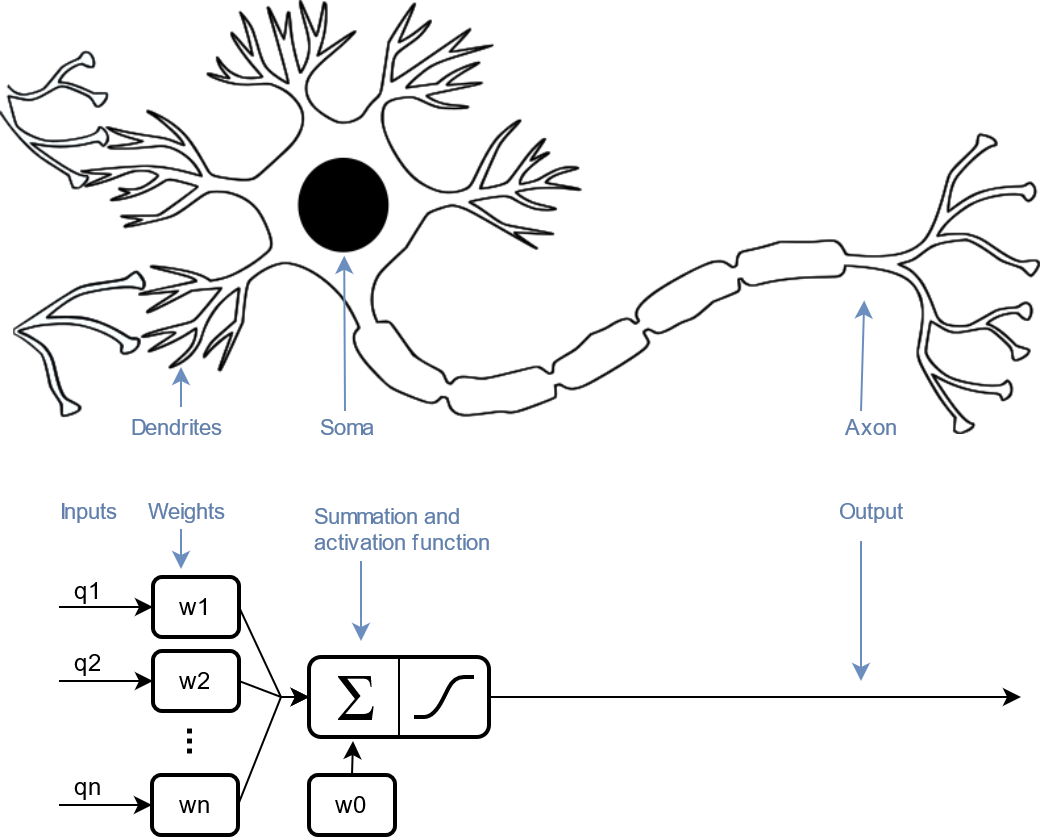
\includegraphics[width=\linewidth]{"../Chap2/Figures/Fig_neuron.png"}
	\caption{The search for “deep learning 3D human pose estimation” (dots) fits an exponential curve (line). The search produced less than 100 results until 2015, and is now well over a 1,000 per year.}
	\label{fig_neuron}
\end{figure}

Schéma draw.io
dendrite input
soma summation function
axon output

Perceptron \cite{Rosenblatt1958}

CNN

Deep learning

- Neurone physiologique recueille les influx nerveux perçus par les dendrites, et si le potentiel dépasse le seuil il déclenche un potentiel d'action envoyé par l'axone vers les neurones suivant.
- Neurone numérique recueille les résultats des filtrages en entrée, les pondère et les somme, et si le résultat dépasse le seuil il déclenche une sortie (roue, voiture, avenue) qu'il envoie au neurone suivant. -> perceptron mono/multicoucheNeurone: unité d'apprentissage



History natural neuron and formal neuron (dates, names, comparison)

Timeline cahier jaune et wiki

S'inspirer de wikipedia (en, fr, timeline); 
S'inspirer du mail machine learning starred (exemple du réseau de neurones); 
S'inspirer du cahier jaune


- deep learning vs CNN (vs SVM, random forest, etc.), AI, machine learning

- classification vs detection vs segmentation

data augmentation, dropout, batch normalization
overfitting
train / test
accuracy loss
gradient descent
layers, batch size, epochs, activation

transfer learning

% \subsection{Application to object detection and localization}


\subsection{Pose detection}

Different architectures, different models, different datasets


\section{3D reconstruction}\label{sec:3D reconstruction}

While some approaches only rely on 2D pose estimation to infer 3D pose with another machine learning model, they are generally not considered to be sufficiently reliable. It is, then, important to use the input from several cameras, and to fuse their informations to obtain 3D coordinates.


\subsection{Pinhole camera model}

Voilà


\subsection{Calibration}

test


\subsection{Triangulation}

suite


\section{3D joint kinematics}

\subsection{Physically consistent model}

autre


\subsection{Scaling}

bref


\subsection{Inverse kinematics}

As opposed to forward kinematics \newline
Compare with 2D angles between 3 points \newline
Different methods (model based vs autres) for angles (cf mail starred)\newline




